\begin{figure}[t]
\centering
\ifbilingual
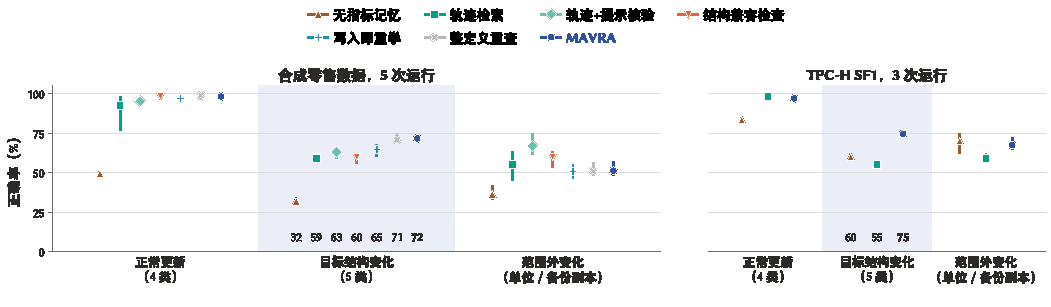
\includegraphics[width=\linewidth]{figures/two-schemas-zh}
\else
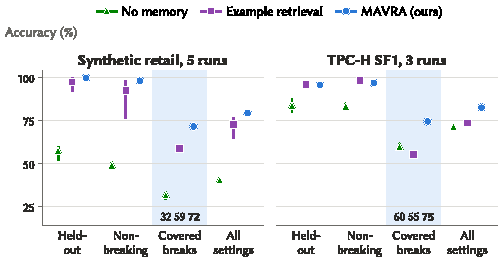
\includegraphics[width=\linewidth]{figures/two-schemas}
\fi
\caption{\bt{Accuracy over held-out questions, eleven changes and cross-agent forms (\PubScenarioScored{} answers). Equal-schema means across all \PubScenarioSettings{} settings: MAVRA \PubJointMAVRAAcc\%, AWM \PubJointAWMAcc\%. One run/method; frozen baseline controls reused.}{留出题、十一种变化及跨智能体题型的正确率（\PubScenarioScored{} 次作答）。两模式及全部 \PubScenarioSettings{} 种情形等权汇总：MAVRA \PubJointMAVRAAcc\%，AWM \PubJointAWMAcc\%。每方法一轮，复用冻结基线对照。}}
\label{fig:twoschemas}
\Description{Compact grouped bars compare ACE, AWM, G-Memory, and full MAVRA on synthetic retail and TPC-H SF1. Questions cover single periods, period differences, highest months and largest monthly increases. Groups show non-breaking updates, covered structural changes, new-agent form transfer, and all settings, on a common zero-to-100-percent scale. All settings also include the original held-out, unit and backup-source cases. Unchanged published baseline controls are reused; the repaired native method and all extra queries are freshly evaluated. Each extra question provides the same explicit business definition to a new agent. No confidence intervals or statistical-significance claim is made.}
\end{figure}
